\documentclass[../main/TOP_manual]{subfiles}

\newcommand{\cd}{\mathrm{CO_2}}
\newcommand{\Ct}{\mathrm{C_T}}
\newcommand{\pacd}{\mathrm{p^a_{CO_2}}}
\newcommand{\cq}{\mathrm{^{14}C}}
\newcommand{\Dcq}{\Delta ^{14}\mathrm{C}}
\newcommand{\Rq}{\mathrm{^{14}{R}}}
\newcommand{\CODE}[1]{\textsc{#1}}
%\newcommand{\CODE}[1]{\textcolor{black}{\textsc{#1}}\xspace}

\begin{document}

\chapter{Model Description}
\label{chap:ModDes}
\chaptertoc

\section{Basics}
\label{sec:Bas}

The time evolution of any passive tracer $C$ follows the transport equation, which is similar to that of active tracer - temperature or salinity :

\begin{equation}
\frac{\partial C}{\partial t} = {S(C)} -  \frac{1}{b_t} \left[   \frac{\partial e_{2u}\,e_{3u} \;  u\, C}{\partial i} +   \frac{\partial e_{1v}\,e_{3v} \;  uv, C}{\partial i}  \right] + \frac{1}{e_{3t}} \frac{\partial w\, C}{\partial k} + D^{lC} + D^{vC}
\label{Eq_tracer}
\end{equation}

where expressions of $D^{lC}$ and $D^{vC}$ depend on the choice for the lateral and vertical subgrid scale parameterizations, see equations 5.10 and 5.11 in \citep{nemo_manual}

{S(C)} , the first term on the right hand side of \ref{Eq_tracer}; is the SMS - Source Minus Sink - inherent to the tracer.  In the case of biological tracer such as phytoplankton, {S(C)} is the balance between phytoplankton growth and its decay through mortality and grazing. In the case of a tracer comprising carbon,  {S(C)} accounts for gas exchange, river discharge, flux to the sediments, gravitational sinking and other biological processes. In the case of a radioactive tracer, {S(C)} is simply loss due to radioactive decay.

The second term (within brackets) represents the advection of the tracer in the three directions. It can be interpreted as the budget between the incoming and outgoing tracer fluxes in a volume $T$-cells $b_t= e_{1t}\,e_{2t}\,e_{3t}$

The third term  represents the change due to lateral diffusion.

The fourth term is change due to vertical diffusion, parameterized as eddy diffusion to represent vertical turbulent fluxes :

\begin{equation}
D^{vC} =  \frac{1}{e_{3t}} \frac{\partial}{\partial k} \left[  A^{vT} \frac{\partial C}{\partial k} \right]
\label{Eq_trczdf}
\end{equation}

where $A^{vT}$ is the vertical eddy diffusivity coefficient of active tracers

\section{The NEMO-TOP interface}
\label{sec:TopInt}

TOP is the NEMO hardwired interface toward biogeochemical models and provide the physical constraints/boundaries for oceanic tracers. It consists of a modular framework to handle multiple ocean tracers, including also a variety of built-in modules.

This component of the NEMO framework allows one to exploit available modules  and further develop a range of applications, spanning from the implementation of a dye passive tracer to evaluate dispersion processes (by means of MY\_TRC), track water masses age (AGE module), assess the ocean interior penetration of persistent chemical compounds (e.g., gases like CFC or even PCBs), up to the full set of equations involving marine biogeochemical cycles.

TOP interface has the following location in the code repository : \path{<repository>/src/TOP/}

and the following modules are available:

% -----------  tableau  ------------------------------------
\begin{itemize}
        \item \textbf{TRP}    	    :    Interface to NEMO physical core for computing tracers transport
        \item \textbf{CFC}	    :    Inert carbon tracers (CFC11,CFC12, SF6)
        \item \textbf{C14}	    :    Radiocarbon passive tracer
        \item \textbf{AGE}	    :    Water age tracking
        \item \textbf{MY\_TRC}  :	Template for creation of new modules and external BGC models coupling
        \item \textbf{PISCES}    :	 Built in BGC model. See \citep{aumont_2015} for a throughout description.
\end{itemize}
%  ----------------------------------------------------------

\section{The transport component : TRP}

The passive tracer transport component  shares the same advection/diffusion routines with the dynamics, with specific treatment of some features like the surface boundary conditions, or the positivity of passive tracers concentrations.

 \subsection{ Advection}
%------------------------------------------namtrc_adv----------------------------------------------------
\nlst{namtrc_adv}
%-------------------------------------------------------------------------------------------------------------
The advection schemes used for the passive tracers are the same than the ones for $T$ and $S$ and described in section 5.1 of \citep{nemo_manual}. The choice of an advection scheme  can be selected independently and  can differ from the ones used for active tracers. This choice is made in the \textit{namtrc\_adv} namelist, by  setting to \textit{true} one and only one of the logicals \textit{ln\_trcadv\_xxx}, the same way of what is done for dynamics.
cen2, MUSCL2, and UBS are not \textit{positive} schemes meaning that negative values can appear in an initially strictly positive tracer field which is advected, implying that false extrema are permitted. Their use is not recommended on passive tracers

 \subsection{ Lateral diffusion}
%------------------------------------------namtrc_ldf----------------------------------------------------
\nlst{namtrc_ldf}
%-------------------------------------------------------------------------------------------------------------
In NEMO v4.0, the passive tracer diffusion has necessarily the same form as the active tracer diffusion, meaning that the numerical scheme must be the same. However the passive tracer mixing coefficient can be chosen as a multiple of the active ones by changing the value of \textit{rn\_ldf\_multi} in namelist \textit{namtrc\_ldf}. The choice of numerical scheme is then set  in the \nam{namtra_ldf}{namtra\_ldf} namelist for the dynamic described in section 5.2 of \citep{nemo_manual}.


%-----------------We also offers the possibility to increase zonal equatorial diffusion for passive tracers by introducing an enhanced zonal diffusivity coefficent in the equatorial domain which can be defined by the equation below :
%-----------------\begin{equation} \label{eq:traqsr_iradiance}
%-----------------Aht  = Aht *  rn_fact_lap * \exp( - \max( 0., z -1000  ) / 1000}  \quad \text{for $L=1$ to $N$}
%-----------------\end{equation}

 \subsection{ Tracer damping}

%------------------------------------------namtrc_dmp----------------------------------------------------
\nlst{namtrc_dmp}
%-------------------------------------------------------------------------------------------------------------

The use of newtonian damping  to climatological fields or observations is also coded, sharing the same routine dans active tracers. Boolean variables are defined in the namelist\_top\_ref to select the tracers on which restoring is applied
Options are defined through the \nam{namtrc_dmp}{namtrc\_dmp} namelist variables. The restoring term is added when the namelist parameter \np{ln\_trcdmp} is set to true. The restoring coefficient is a three-dimensional array read in a file, which name is specified by the namelist variable \np{cn\_resto\_tr}. This netcdf file can be generated using the DMP\_TOOLS tool.

 \subsection{ Tracer positivity}

%------------------------------------------namtrc_rad----------------------------------------------------
\nlst{namtrc_rad}
%-------------------------------------------------------------------------------------------------------------

Sometimes, numerical scheme can generates negative values of passive tracers concentration that must be positive. For exemple,  isopycnal diffusion can created extrema. The trcrad routine artificially corrects negative concentrations with a very crude solution that either sets negative concentration to zero without adjusting the tracer budget, or by removing negative concentration and keeping mass conservation.
The treatment of negative concentrations is an option and can be selected in the namelist \nam{namtrc_rad}{namtrc\_rad} by setting the parameter \np{ln\_trcrad}  to true.

\section{The SMS modules}

\label{SMS_models}
%------------------------------------------namtrc_sms----------------------------------------------------
%\nlst{namtrc}
%-------------------------------------------------------------------------------------------------------------

\subsection{Ideal Age}
%------------------------------------------namage----------------------------------------------------
%
\nlst{namage}
%----------------------------------------------------------------------------------------------------------


 An `ideal age' tracer is integrated online in TOP when \textit{ln\_age} = \texttt{.true.} in namelist \textit{namtrc}. This tracer marks the length of time in units of years that fluid has spent in the interior of the ocean, insulated from exposure to the atmosphere. Thus, away from the surface for $z<-H_{\mathrm{Age}}$ where $H_{\mathrm{Age}}$ is specified by the \textit{namage} namelist variable \textit{rn\_age\_depth}, whose default value is 10~m, there is a source $\mathrm{SMS_{\mathrm{Age}}}$ of the age tracer $A$:
\begin{equation}
  \label{eq:TOP-age-interior}
  \mathrm{SMS_{\mathrm{Age}}} = 1 \mathrm{yr}\;^{-1} = 1/T_{\mathrm{year}},
 \end{equation}
 where the length of the current year $T_{\mathrm{year}} = 86400*N_{\mathrm{days\;in\;current\; year}}\;\mathrm{s}$, where $N_{\mathrm{days\;in\;current\; year}}$ may be 366 or 365 depending on whether the current year is a leap year or not.
 Near the surface, for $z>-H_{\mathrm{Age}}$, ideal age is relaxed back to zero:
\begin{equation}
  \label{eq:TOP-age-surface}
   \mathrm{SMS_{\mathrm{Age}}} = -\lambda_{\mathrm{Age}}A,
 \end{equation}
 where the relaxation rate $\lambda_{\mathrm{Age}}$  (units $\mathrm{s}\;^{-1}$) is specified by the \textit{namage} namelist variable \textit{rn\_age\_kill\_rate} and has a default value of 1/7200~s. Since this relaxation is applied explicitly, this relaxation rate in principle should not exceed $1/\Delta t$, where $\Delta t$ is the time step used to step forward passive tracers (2 * \textit{nn\_dttrc * rn\_rdt} when the default  leapfrog time-stepping scheme is employed).

 Currently the 1-dimensional reference depth of the grid boxes is used rather than the dynamically evolving depth to determine whether the age tracer is incremented or relaxed to zero. This means that the tracer only works correctly in z-coordinates. To ensure that the forcing is independent of the level thicknesses, where the tracer cell at level $k$ has its upper face $z=-depw(k)$ above the depth $-H_{\mathrm{Age}}$, but its lower face $z=-depw(k+1)$ below that depth, then the age source
 \begin{equation}
  \label{eq:TOP-age-mixed}
   \mathrm{SMS_{\mathrm{Age}}} = -f_{\mathrm{kill}}\lambda_{\mathrm{Age}}A +f_{\mathrm{add}}/T_{\mathrm{year}} ,
 \end{equation}
 where
 \begin{align}
    f_{\mathrm{kill}} &= e3t_k^{-1}(H_{\mathrm{Age}} - depw(k)) , \\
    f_{\mathrm{add}} &= 1 - f_{\mathrm{kill}}.
 \end{align}


 This implementation was first used in the CORE-II intercomparison runs described e.g.\ in \citet{danabasoglu_2014}.

\subsection{Inert carbons tracer}

%------------------------------------------namage----------------------------------------------------
%
\nlst{namcfc}
%----------------------------------------------------------------------------------------------------------

Chlorofluorocarbons 11 and 12 (CFC-11 and CFC-12), and sulfur hexafluoride (SF6), are synthetic chemicals manufactured for industrial and domestic applications from the early 20th century onwards.
CFC-11 (CCl$_{3}$F) is a volatile liquid at room temperature, and was widely used in refrigeration. CFC-12 (CCl$_{2}$F$_{2}$) is a gas at room temperature, and, like CFC-11, was widely used as a refrigerant,
and additionally as an aerosol propellant. SF6 (SF$_{6}$) is also a gas at room temperature, with a range of applications based around its property as an excellent electrical insulator (often replacing more toxic alternatives).
All three are relatively inert chemicals that are both non-toxic and non-flammable, and their wide use has led to their accumulation within the Earth's atmosphere. Large-scale production of CFC-11 and CFC-12 began in the 1930s, while production of SF6 began in the 1950s, and their atmospheric concentration time-histories are shown in Figure \ref{img_cfcatm}.
As can be seen in the figure, while the concentration of SF6 continues to rise to the present  day, the concentrations of both CFC-11 and CFC-12 have levelled off and declined since around the 1990s.
These declines have been driven by the Montreal Protocol (effective since August 1989), which has banned the production of CFC-11 and CFC-12 (as well as other CFCs) because of their role in the depletion of
stratospheric ozone (O$_{3}$), critical in decreasing the flux of ultraviolet radiation to the Earth's surface. Separate to this role in ozone-depletion, all three chemicals are significantly more potent greenhouse gases
than CO$_{2}$ (especially SF6), although their relatively low atmospheric concentrations limit their role in climate change. \\

% Chlorofluorocarbons 11 and 12 (CFC-11 and CFC-12), and sulfur hexafluoride (SF6),
% are greenhouse gases that have been released into the atmosphere by human activities.
% In the case of CFC-11 and CFC-12, this release began in the 1930s, and atmospheric
% concentrations increased until around the late 1990s afterwhich they began to decline in
% response to the Montreal Protocol.
% In the case of SF6, release began in the 1950s
% This release began in the 1930s for CFC-11 and CFC-12, and the 1950s for SF6, and
% regularly increasing their atmospheric concentration until the 1090s, 2000s for respectively CFC11, CFC12,
% and is still increasing, and SF6 (see Figure \ref{img_cfcatm}).  \\

The ocean is a notable sink for all three gases, and their relatively recent occurrence in the atmosphere, coupled to the ease of making high precision measurements of their dissolved concentrations, has made them
valuable in oceanography. % for tracking interior ventilation and mixing.
Because they only enter the ocean via surface air-sea exchange, and are almost completely chemically and biologically inert, their distribution within the ocean interior reveals its ventilation via transport and mixing.
Measuring the dissolved concentrations of the gases -- as well as the mixing ratios between them -- shows circulation pathways within the ocean as well as water mass ages (i.e. the time since last contact with the
atmosphere). This feature of the gases has made them valuable across a wide range of oceanographic problems. One use lies in ocean modelling, where they can be used to evaluate the realism of the circulation and
ventilation of models, key for understanding the behaviour of wider modelled marine biogeochemistry (e.g. \citep{dutay_2002,palmieri_2015}). \\

Modelling these gases (henceforth CFCs) in NEMO is done within the passive tracer transport module, TOP, using the conservation state equation \ref{Eq_tracer}

Advection and diffusion of the CFCs in NEMO are calculated by the physical module, OPA,
whereas sources and sinks are done by the CFC module within TOP.
The only source for CFCs in the ocean is via air-sea gas exchange at its surface, and since CFCs are generally
stable within the ocean, we assume that there are no sinks (i.e. no loss processes) within the ocean interior.
Consequently, the sinks-minus-sources term for CFCs consists only of their air-sea fluxes, $F_{cfc}$, as
described in the Ocean Model Inter-comparison Project (OMIP) protocol \citep{orr_2017}:

% Because CFCs being stable in the ocean, we consider that there is no CFCs sink.
% The only CFC source in the ocean is through the Air-Sea gas exchange at the surface.
% These are calculated as air-sea fluxes (F$_{cfc}$), as described in the OMIP6 protocol \citep{artOMIP6}:

\begin{eqnarray}
F_{cfc} = K_{w} \, \cdot \, (C_{sat} - C_{surf}) \, \cdot  \, (1 - f_{i})
\label{equ_CFC_flux}
\end{eqnarray}

Where $K_{w}$ is the piston velocity (in m~s$^{-1}$), as defined in Equation \ref{equ_Kw};
$C_{sat}$ is the saturation concentration of the CFC tracer, as defined in Equation \ref{equ_C_sat};
$C_{surf}$ is the local surface concentration of the CFC tracer within the model (in mol~m$^{-3}$);
and $f_{i}$ is the fractional sea-ice cover of the local ocean (ranging between 0.0 for ice-free ocean,
through to 1.0 for completely ice-covered ocean with no air-sea exchange).

The saturation concentration of the CFC, $C_{sat}$, is calculated as follows:

\begin{eqnarray}
C_{sat} = Sol \, \cdot \, P_{cfc}
\label{equ_C_sat}
\end{eqnarray}

Where $Sol$ is the gas solubility in mol~m$^{-3}$~pptv$^{-1}$, as defined in Equation \ref{equ_Sol_CFC};
and $P_{cfc}$ is the atmosphere concentration of the CFC (in parts per trillion by volume, pptv).
This latter concentration is provided to the model by the historical time-series of \citet{bullister_2017}.
This includes bulk atmospheric concentrations of the CFCs for both hemispheres -- this is necessary because of
the geographical asymmetry in the production and release of CFCs to the atmosphere.
Within the model, hemispheric concentrations are uniform, with the exception of the region between
10$^{\circ}$N and 10$^{\circ}$ in which they are linearly interpolated.

The piston velocity $K_{w}$ is a function of 10~m wind speed (in m~s$^{-1}$) and sea surface temperature,
$T$ (in $^{\circ}$C), and is calculated here following \citet{wanninkhof_1992}:

\begin{eqnarray}
K_{w} = X_{conv} \, \cdot \, a \, \cdot \, u^2 \, \cdot \, \sqrt{ \frac{Sc(T)}{660} }
\label{equ_Kw}
\end{eqnarray}

Where $X_{conv}$ = $\frac{0.01}{3600}$, a conversion factor that changes the piston velocity
from cm~h$^{-1}$ to m~s$^{-1}$;
$a$ is a constant re-estimated by \citet{wanninkhof_2014} to 0.251 (in $\frac{cm~h^{-1}}{(m~s^{-1})^{2}}$);
and $u$ is the 10~m wind speed in m~s$^{-1}$ from either an atmosphere model or reanalysis atmospheric forcing.
$Sc$ is the Schmidt number, and is calculated as follow, using coefficients from \citet{wanninkhof_2014} (see Table \ref{tab_Sc}).

\begin{eqnarray}
Sc =  a0 + (a1 \, \cdot \, T) + (a2  \, \cdot \, T^2) + (a3 \, \cdot \, T^3) + (a4 \, \cdot \, T^4)
\label{equ_Sc}
\end{eqnarray}

The solubility, $Sol$, used in Equation \ref{equ_C_sat} is calculated in mol~l$^{-1}$~atm$^{-1}$,
and is specific for each gas.
It has been experimentally estimated by \citet{warner_1985} as a function of temperature
and salinity:

% AXY: this equation looks both weird and possibly wrong; it doesn't look like the one in the
% code version that I have to hand, although this might be out of date; in any case, I'dag
% strongly suggest avoiding the use of the \frac{}{100}, and instead substitute a term that is
% "degrees Kelvin divided by 100" (which is weird in itself); and make this term use Celcius
% so that you're not using T twice in different ways

\begin{eqnarray}
\ln{(Sol)} = a_1 + \frac{a_2}{ T_{X}} + a_3 \, \cdot \, \ln{ T_{X} } + a_4 \, \cdot \, T_{X}^2 + S \, \cdot \, ( b_1 + b_2 \, \cdot \, T_{X} + b_3 \, \cdot \, T_{X}^2 )
\label{equ_Sol_CFC}
\end{eqnarray}

% \begin{eqnarray}
% \ln{(Sol)} = a1 + a2 \, \frac{100}{T} + a3 \, \ln{ (\frac{T}{100}) } + a4 \, \frac{T}{100}^2 + S \, ( b1 + b2 \, \frac{T}{100} + b3 \, \frac{T}{100}^2 )
% \label{equ_Sol_CFC}
% \end{eqnarray}

Where $T_{X}$ is $\frac{T + 273.16}{100}$, a function of temperature;
and the $a_{x}$ and $b_{x}$ coefficients are specific for each gas (see Table \ref{tab_ref_CFC}).
This is then converted to mol~m$^{-3}$~pptv$^{-1}$ assuming a constant atmospheric surface pressure of 1~atm.
The solubility of CFCs thus decreases with rising $T$ while being relatively insensitive to salinity changes.
Consequently, this translates to a pattern of solubility where it is greatest in cold, polar regions (see Figure \ref{img_cfcsol}).

% AXY: not 100% sure about the units below; they might be in nanomol, or in seconds or years

The standard outputs of the CFC module are seawater CFC concentrations (in mol~m$^{-3}$), the net air-sea flux (in mol~m$^{-2}$~d$^{-1}$) and the cumulative net air-sea flux (in mol~m$^{-2}$).
Using XIOS, it is possible to obtain outputs such as the vertical integral of CFC concentrations (in mol~m$^{-2}$; see Figure \ref{img_cfcinv}).
This property, when divided by the surface CFC concentration, estimates the local penetration depth (in m) of the CFC.

% AXY: not sure what's meant by some of the below; I've tried to reword it above
% The standard outputs of the CFC module are the CFCs concentration in the sea water, and the records of the outputs-frequency-averaged as well as the total air-sea fluxes.
% Using XIOS, it is also possible to ask for the CFCs vertical inventory in the output file (see Figure cfc inventory example ?).

\subsubsection{Notes}

In comparison to the OMIP protocol, the CFC module in NEMO has several differences:

% AXY: consider an itemized list here if you've got a list of differences

For instance, C$_{sat}$ is calculated for a fixed surface pressure of 1atm, what could be corrected in a further version of the module.


\begin{table}[!t]
\caption{Coefficients for fit of the CFCs solubility (Eq. \ref{equ_Sol_CFC}).}
\vskip4mm
\centering
\begin{tabular}{l l l l l l l l l}
\hline
Gas   & & a1 & a2 & a3 & a4 & b1 & b2 & b3 \\
\hline
CFC-11 & & -218.0971 & 298.9702 & 113.8049 & -1.39165 & -0.143566  & 0.091015   & -0.0153924 \\
CFC-12 & & -229.9261 & 319.6552 & 119.4471 & -1.39165 & -0.142382  & 0.091459   & -0.0157274 \\
SF6    & & -80.0343  & 117.232  & 29.5817  & 0.0      & 0.0335183  & -0.0373942 & 0.00774862 \\
\hline
\end{tabular}
\label{tab_ref_CFC}
\end{table}


\begin{table}[!t]
\caption{Coefficients for fit of the CFCs Schmidt number (Eq. \ref{equ_Sc}). }
\vskip4mm
\centering
\begin{tabular}{l l l l l l l }
\hline
Gas  & & a0 & a1 & a2 & a3 & a4 \\
\hline
CFC-11 & & 3579.2  & -222.63 & 7.5749 & -0.14595 & 0.0011874   \\
CFC-12 & & 3828.1  & -249.86 & 8.7603 & -0.1716  & 0.001408    \\
SF6    & & 3177.5  & -200.57 & 6.8865 & -0.13335 & 0.0010877   \\
\hline
\end{tabular}
\label{tab_Sc}
\end{table}

%% -----------------------------------
%% -----------------------------------
%% Figures %%


\begin{figure}[!h]
\centering
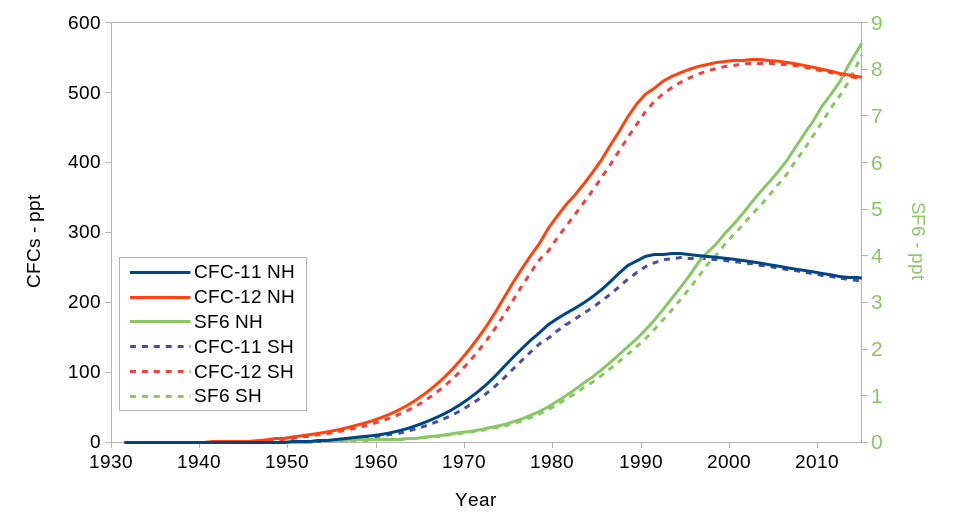
\includegraphics[width=0.80\textwidth]{CFC-atm-evol}
  \caption{Atmospheric CFC11, CFC12 and SF6 partial pressure evolution in both hemispheres.}
\label{img_cfcatm}
\end{figure}

\begin{figure}[!h]
\centering
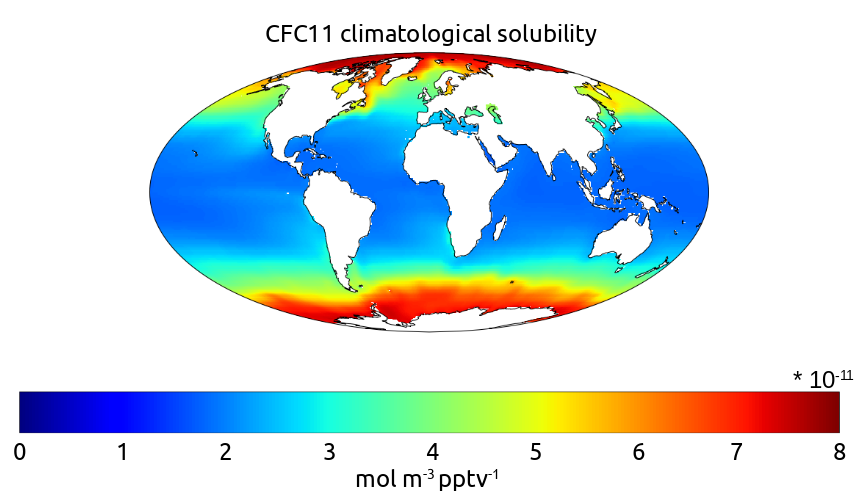
\includegraphics[width=0.80\textwidth]{CFC_solub}
  \caption{CFC11 solubility in mol m$^{-3}$ pptv$^{-1}$, calculated from the World Ocean Atlas 2013 temperature and salinity annual climatology.}
\label{img_cfcsol}
\end{figure}

\begin{figure}[!h]
\centering
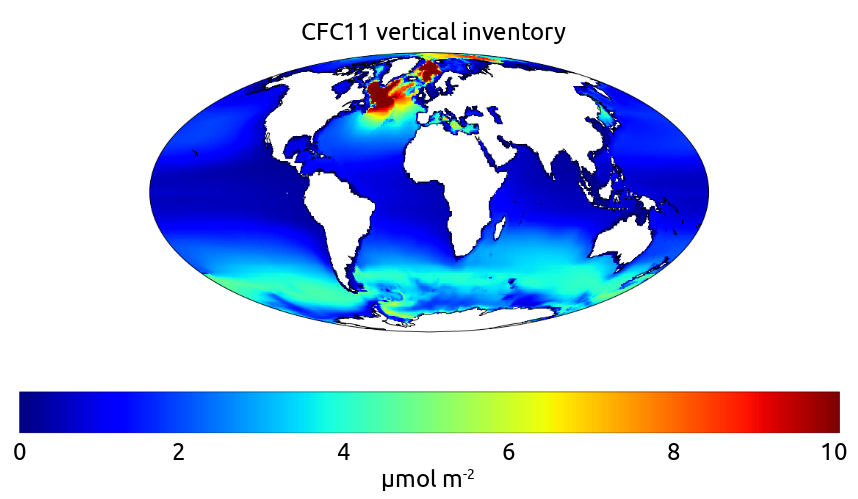
\includegraphics[width=0.80\textwidth]{CFC_inventory}
  \caption{CFC11 vertical inventory in $\mu$mol m$^{-2}$, from one of the UK Earth System Model 1 model (UKESM1 - which uses NEMO as ocean component, with TOP for the passive tracers) historical run at year 2000.}
\label{img_cfcinv}
\end{figure}


\subsection{Radiocarbon}

%------------------------------------------namage----------------------------------------------------
%
\nlst{namc14_fcg}
\nlst{namc14_typ}
\nlst{namc14_sbc}
%----------------------------------------------------------------------------------------------------------

The C14 package implemented in NEMO by Anne Mouchet models ocean $\Dcq$. It offers several possibilities: $\Dcq$ as a physical tracer of the ocean ventilation (natural $\cq$), assessment of bomb radiocarbon uptake, as well as transient studies of paleo-historical ocean radiocarbon distributions.

\subsubsection{Method}

 Let  $\Rq$ represent the ratio of $\cq$ atoms to the total number of carbon atoms in the sample, i.e. $\cq/\mathrm{C}$. Then, radiocarbon anomalies are reported as
\begin{equation}
\Dcq = \left( \frac{\Rq}{\Rq_\mathrm{ref}} - 1 \right) 10^3, \label{eq:c14dcq}
\end{equation}
where $\Rq_{\textrm{ref}}$ is a reference ratio. For the purpose of ocean ventilation studies $\Rq_{\textrm{ref}}$ is set to one.

Here we adopt the approach of \cite{fiadeiro_1982} and \cite{toggweiler_1989a,toggweiler_1989b} in which  the ratio $\Rq$ is transported rather than the individual concentrations C and $\cq$.
This approach calls for a strong assumption, i.e., that of a homogeneous and constant dissolved inorganic carbon (DIC) field \citep{toggweiler_1989a,mouchet_2013}. While in terms of
oceanic $\Dcq$, it yields similar results to approaches involving carbonate chemistry, it underestimates the bomb radiocarbon inventory because it assumes a constant air-sea $\cd$ disequilibrium (Mouchet, 2013). Yet, field reconstructions of the ocean bomb $\cq$ inventory are also biased low \citep{naegler_2009} since they assume that the anthropogenic perturbation did not affect ocean DIC since the pre-bomb epoch. For these reasons, bomb $\cq$ inventories obtained with the present method are directly comparable to reconstructions based on field measurements.

This simplified approach also neglects the effects of fractionation (e.g.,  air-sea exchange) and of biological processes. Previous studies by \cite{bacastow_1990} and \cite{joos_1997} resulted in nearly identical $\Dcq$ distributions among experiments considering biology or not.
Since observed $\Rq$ ratios are corrected for the isotopic fractionation when converted to the standard $\Dcq$ notation \citep{stuiver_1977} the model results are directly comparable to observations.

Therefore the simplified approach is justified for the purpose of assessing the circulation and ventilation of OGCMs.

The equation governing the transport of $\Rq$  in the ocean is
\begin{equation}
\frac{\partial}{\partial t} {\Rq} =  - \bigtriangledown \cdot ( \mathbf{u} \Rq - \mathbf{K} \cdot \bigtriangledown \Rq )  - \lambda \Rq, \label{eq:quick}
\end{equation}
where $\lambda$ is the radiocarbon decay rate, ${\mathbf{u}}$ the 3-D velocity field, and $\mathbf{K}$ the diffusivity tensor.

At the air-sea interface a Robin boundary condition \citep{haine_2006} is applied to \eqref{eq:quick}, i.e., the flux
through the interface is proportional to the difference in the ratios between
the ocean and the atmosphere
\begin{equation}
\mathcal{\!F} =  \kappa_{R}  (\Rq  - \Rq_{a} ), \label{eq:BCR}
\end{equation}
where $\mathcal{\!F}$ is the flux out of the ocean, and $\Rq_{a}$ is the atmospheric $\cq/\mathrm{C}$ ratio. The transfer velocity $ \kappa_{R} $ for the radiocarbon ratio in \eqref{eq:BCR} is computed as
\begin{equation}
 \kappa_{R} =  \frac{\kappa_{\cd} K_0}{\overline{\Ct}} \, \pacd   \label{eq:Rspeed}
\end{equation}
with $\kappa_{\cd}$ the carbon dioxide transfer or piston velocity, $K_0$ the $\cd$ solubility in seawater, $\pacd$ the atmospheric $\cd$ pressure at sea level, and $\overline{\Ct}$ the average sea-surface dissolved inorganic carbon concentration.


The $\cd$ transfer velocity is based on the empirical formulation of \cite{wanninkhof_1992} with chemical enhancement \citep{wanninkhof_1996,wanninkhof_2014}. The original formulation is modified to account for the reduction of the  air-sea exchange rate in the presence of sea ice. Hence
\begin{equation}
\kappa_\cd=\left( K_W\,\mathrm{w}^2 + b  \right)\, (1-f_\mathrm{ice})\,\sqrt{660/Sc}, \label{eq:wanc14}
\end{equation}
with $\mathrm{w}$ the wind magnitude, $f_\mathrm{ice}$ the fractional ice cover, and $Sc$ the Schmidt number.
$K_W$ in \eqref{eq:wanc14} is an empirical coefficient with dimension of an inverse velocity.
The chemical enhancement term $b$ is represented as a function of temperature $T$ \citep{wanninkhof_1992}
\begin{equation}
b=2.5 ( 0.5246 + 0.016256 T+ 0.00049946  * T^2 ). \label{eq:wanchem}
\end{equation}

%We compare the results of equilibrium and transient experiments obtained with both methods in section \ref{sec:UNDEU}.

%
\subsubsection{Model setup}
\label{sec:setup}

To activate the \texttt{C14} package, set the parameter \textit{ln\_c14} = \texttt{.true.} in namelist \textit{namtrc}.

\paragraph{Parameters and formulations}
\label{sec:param}
 %
The radiocarbon decay rate (\CODE{rlam14}; in \texttt{trcnam\_c14} module) is set to $\lambda=(1/8267)$ yr$^{-1}$ \citep{stuiver_1977}, which corresponds to a half-life of 5730 yr.\\[1pt]
%
The Schmidt number $Sc$, Eq. \eqref{eq:wanc14}, is calculated with the help of the formulation of \cite{wanninkhof_2014}. The $\cd$ solubility $K_0$ in \eqref{eq:Rspeed} is taken from \cite{weiss_1974}. $K_0$ and $Sc$ are computed with the OGCM temperature and salinity fields (\texttt{trcsms\_c14} module).\\[1pt]
%
The following parameters intervening in the air-sea exchange rate are set in \texttt{namelist\_c14}:
\begin{itemize}
\item The reference DIC concentration $\overline{\Ct}$ (\CODE{xdicsur}) intervening in \eqref{eq:Rspeed} is classically set to 2 mol m$^{-3}$ \citep{toggweiler_1989a,orr_2001,butzin_2005}.
%
\item The value of the empirical coefficient $K_W$ (\CODE{xkwind}) in \eqref{eq:wanc14} depends on the wind field and on the model upper ocean mixing rate \citep{toggweiler_1989a,wanninkhof_1992,naegler_2009,wanninkhof_2014}.
It should be adjusted so that the globally averaged $\cd$ piston velocity is $\kappa_\cd = 16.5\pm 3.2$ cm/h \citep{naegler_2009}.
%The sensitivity to this parametrization is discussed in section \ref{sec:result}.
%
\item Chemical enhancement (term $b$  in Eq. \ref{eq:wanchem}) may be set on/off by means of the logical variable \CODE{ln\_chemh}.
\end{itemize}

%
\paragraph{Experiment type}
The type of experiment is determined by the value given to \CODE{kc14typ} in \texttt{namelist\_c14}. There are three possibilities:
\begin{enumerate}
\item natural $\Dcq$: \CODE{kc14typ}=0
\item bomb $\Dcq$: \CODE{kc14typ}=1
\item transient paleo-historical $\Dcq$: \CODE{kc14typ}=2
\end{enumerate}
%
\textbf{Natural or Equilibrium radiocarbon}
\CODE{kc14typ}=0

Unless otherwise specified in \texttt{namelist\_c14}, the atmospheric $\Rq_a$ (\CODE{rc14at}) is set to one, the atmospheric $\cd$ (\CODE{pco2at}) to 280 ppm, and the ocean $\Rq$ is initialized with \CODE{rc14init=0.85}, i.e., $\Dcq=$-150\textperthousand  \cite[typical for deep-ocean, Fig 6 in][]{key_2004}.

Equilibrium experiment should last until 98\% of the ocean volume exhibit a drift of less than 0.001\textperthousand/year \citep{orr_2000}; this is usually achieved after few kyr (Fig. \ref{fig:drift}).
%
\begin{figure}[!h]
\begin{center}
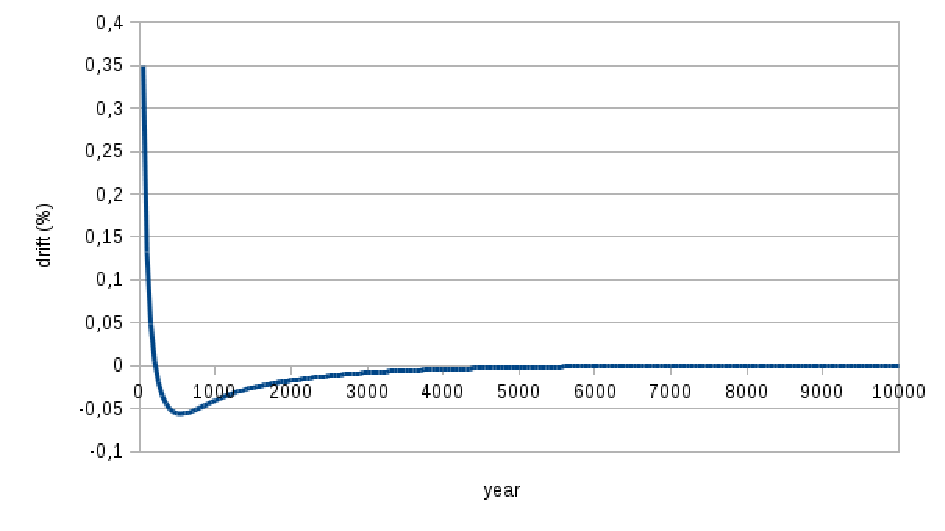
\includegraphics[width=0.9\hsize]{drift-EXP06}
\end{center}
\vspace{-4ex}
\caption{ Time evolution of $\Rq$ inventory anomaly for equilibrium run with homogeneous ocean initial state. The anomaly (or drift) is given in \%  change in total ocean inventory per 50 years. Time on x-axis is in simulation year.\label{fig:drift} }
\end{figure}

\textbf{Transient: Bomb}
\label{sec:bomb}
\CODE{kc14typ}=1

\begin{figure}[!h]
\begin{center}
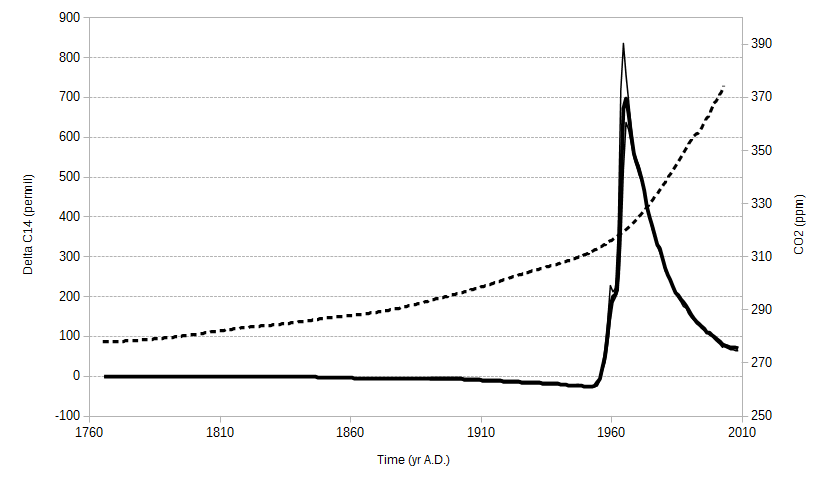
\includegraphics[width=0.9\hsize]{C14bombCO2-NB}
\end{center}
\vspace{-4ex}
\caption{Atmospheric $\Dcq$ (solid; left axis) and $\cd$ (dashed; right axis)  forcing for the $\cq$-bomb experiments. The $\Dcq$ is illustrated for the three zonal bands (upper, middle, and lower curves correspond to latitudes $> 20$N, $\in [20\mathrm{S},20\mathrm{N}]$, and $< 20$S, respectively.} \label{fig:bomb}
\end{figure}

Performing this type of experiment requires that a pre-industrial equilibrium run be performed beforehand (\CODE{ln\_rsttr} should be set to \texttt{.TRUE.}).

An exception to this rule is when wishing to perform a perturbation bomb experiment as was possible with the package \texttt{C14b}. It is still possible to easily set-up that type of transient experiment for which no previous run is needed.  In addition to the instructions as given in this section it is however necessary to adapt the \texttt{atmc14.dat} file so that it does no longer contain any negative $\Dcq$ values (Suess effect in the pre-bomb period).

The model  is integrated from a given initial date following the observed records provided from 1765 AD on ( Fig. \ref{fig:bomb}).
The file \texttt{atmc14.dat}  \cite[][\& I. Levin, personal comm.]{enting_1994} provides atmospheric $\Dcq$ for three latitudinal bands: 90S-20S,    20S-20N \&    20N-90N.
Atmospheric $\cd$ in the file \texttt{splco2.dat} is obtained from a spline fit through ice core data and direct atmospheric measurements \cite[][\& J. Orr, personal comm.]{orr_2000}.
Dates in these forcing files are expressed as yr AD.

To ensure that the atmospheric forcing is applied properly as well as that output files contain consistent dates and inventories the experiment should be set up carefully:
\begin{itemize}
\item Specify the starting date of the experiment: \CODE{nn\_date0} in \texttt{namelist}.  \CODE{nn\_date0} is written as Year0101 where Year may take any positive value (AD).
\item Then the parameters \CODE{nn\_rstctl} in  \texttt{namelist} (on-line) and \CODE{nn\_rsttr} in \texttt{namelist\_top} (off-line)  must be \textbf{set to 0} at the start of the experiment (force the date to \CODE{nn\_date0} for the \textbf{first} experiment year).
\item These two parameters (\CODE{nn\_rstctl} and \CODE{nn\_rsttr}) have then to be \textbf{set to 2} for the following years (the date must be read in the restart file).
\end{itemize}
 If the experiment date is outside the data time span then the first or last atmospheric concentrations are prescribed depending on whether the date is earlier or later. Note that \CODE{tyrc14\_beg} (\texttt{namelist\_c14}) is not used in this context.

%
\textbf{Transient: Past}
\CODE{kc14typ}=2
%
\begin{figure}[!h]
\begin{center}
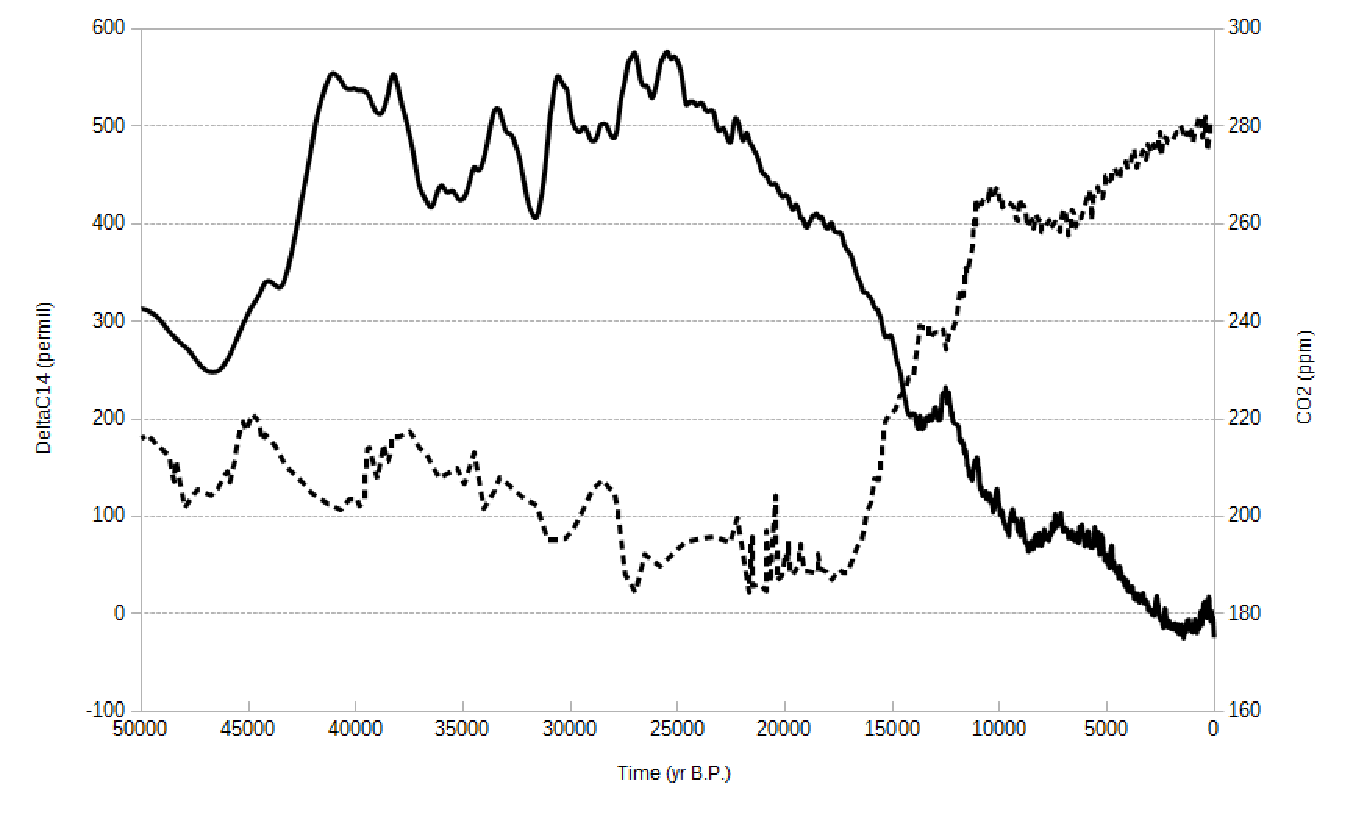
\includegraphics[width=0.9\hsize]{PaleoCO2C14-NB}
\end{center}
\vspace{-4ex}
\caption{Atmospheric $\Dcq$ (solid) and $\cd$ (dashed)  forcing for the Paleo experiments. The $\cd$ scale is given on the right axis.} \label{fig:paleo}
\end{figure}

This experiment type does not need a previous equilibrium run. It should start 5--6 kyr earlier than the period to be analyzed.
Atmospheric $\Rq_a$ and $\cd$ are prescribed from forcing files. The ocean $\Rq$ is initialized with the value attributed to \CODE{rc14init} in \texttt{namelist\_c14}.

The file \texttt{intcal13.14c} \citep{reimer_2013} contains atmospheric $\Dcq$ from 0 to 50 kyr cal BP\footnote{cal BP: number of years before 1950 AD}.
The $\cd$ forcing is provided in file \texttt{ByrdEdcCO2.txt}. The content of this file is based on  the high resolution record from EPICA Dome C \citep{monnin_2004} for the Holocene and the Transition, and on Byrd Ice Core CO2 Data for 20--90 kyr BP  \citep{ahn_2008}. These atmospheric values are reproduced in Fig. \ref{fig:paleo}. Dates in these files are expressed as yr BP.

To ensure that the atmospheric forcing is applied properly as well as that output files contain consistent dates and inventories the experiment should be set up carefully.
The true experiment starting date is given by \CODE{tyrc14\_beg} (in yr BP) in \texttt{namelist\_c14}. In consequence, \CODE{nn\_date0} in \texttt{namelist} MUST be set to 00010101.\\
Then the parameters \CODE{nn\_rstctl} in  \texttt{namelist} (on-line) and \CODE{nn\_rsttr} in \texttt{namelist\_top} (off-line)  must be set to 0 at the start of the experiment (force the date to \CODE{nn\_date0} for the first experiment year). These two parameters have then to be set to 2 for the following years (read the date in the restart file). \\
 If the experiment date is outside the data time span then the first or last atmospheric concentrations are prescribed depending on whether the date is earlier or later.

%
\paragraph{Model output}
\label{sec:output}
All output fields in Table \ref{tab:out} are routinely computed. It depends on the actual settings in \texttt{iodef.xml} whether they are stored or not.
%
\begin{table}[!h]
\begin{center}
\caption{Standard output fields for the C14 package \label{tab:out}.
}
%\begin{small}
\renewcommand{\arraystretch}{1.3}%
\begin{tabular}[h]{|l*{3}{|c}|l|}
\hline
Field & Type & Dim & Units & Description \\ \hline
RC14 & ptrc & 3-D & -        & Radiocarbon ratio \\
DeltaC14 & diad & 3-D & \textperthousand & $\Dcq$\\
C14Age & diad & 3-D & yr &   Radiocarbon age \\
RAge & diad & 2-D & yr & Reservoir age\\
qtr\_c14 &  diad & 2-D & m$^{-2}$ yr$^{-1}$ & Air-to-sea net $\Rq$ flux\\
qint\_c14 & diad & 2-D &   m$^{-2}$ &  Cumulative air-to-sea $\Rq$ flux \\
AtmCO2 & scalar & 0-D & ppm & Global atmospheric $\cd$ \\
AtmC14 & scalar & 0-D & \textperthousand  & Global atmospheric $\Dcq$\\
K\_CO2 & scalar & 0-D & cm h$^{-1}$  & Global $\cd$ piston velocity ($ \overline{\kappa_{\cd}}$) \\
K\_C14 & scalar & 0-D &m yr$^{-1}$ & Global $\Rq$ transfer velocity  ($ \overline{\kappa_R}$)\\
C14Inv & scalar & 0-D & $10^{26}$ atoms & Ocean radiocarbon inventory \\ \hline
\end{tabular}
%\end{small}
\end{center}
\end{table}
%!   Standard ratio: 1.176E-12 ; Avogadro's nbr = 6.022E+23 at/mol ; bomb C14 traditionally reported as 1.E+26 atoms
%   REAL(wp), PARAMETER            :: atomc14=1.176*6.022E-15   ! conversion factor
% atomc14 * xdicsur * zdum

The radiocarbon age is computed as  $(-1/\lambda) \ln{ \left( \Rq \right)}$, with zero age corresponding to $\Rq=1$.

The reservoir age is the age difference between the ocean uppermost layer and the atmosphere. It is usually reported as conventional radiocarbon age; i.e., computed by means of the Libby radiocarbon mean life \cite[8033 yr;][]{stuiver_1977}
\begin{align}
{^{14}\tau_\mathrm{c}}= -8033 \; \ln \left(1 + \frac{\Dcq}{10^3}\right), \label{eq:convage}
\end{align}
where ${^{14}\tau_\mathrm{c}}$ is expressed in years B.P. Here we do not use that convention and compute reservoir ages with the mean lifetime $1/\lambda$. Conversion from one scale to the other is readily performed. The conventional radiocarbon age is lower than the radiocarbon age by $\simeq3\%$.

The ocean radiocarbon  inventory is computed as
\begin{equation}
N_A \Rq_\mathrm{oxa} \overline{\Ct} \left( \int_\Omega \Rq d\Omega \right) /10^{26}, \label{eq:inv}
\end{equation}
where $N_A$ is the Avogadro's number ($N_A=6.022\times10^{23}$ at/mol), $\Rq_\mathrm{oxa}$ is the oxalic acid radiocarbon standard \cite[$\Rq_\mathrm{oxa}=1.176\times10^{-12}$;][]{stuiver_1977}, and $\Omega$ is the ocean volume.  Bomb $\cq$ inventories are traditionally reported in units of $10^{26}$ atoms, hence the denominator in \eqref{eq:inv}.

All transformations from second to year, and inversely, are performed with the help of the physical constant \CODE{rsiyea} the sideral year length expressed in seconds\footnote{The variable (\CODE{nyear\_len}) which reports the length in days of the previous/current/future year (see \textrm{oce\_trc.F90}) is not a constant. }.

The global transfer velocities represent time-averaged\footnote{the actual duration is set in \texttt{iodef.xml}} global integrals of the transfer rates:
 \begin{equation}
 \overline{\kappa_{\cd}}= \int_\mathcal{S} \kappa_{\cd} d\mathcal{S}  \text{ and } \overline{\kappa_R}= \int_\mathcal{S} \kappa_R d\mathcal{S}
\end{equation}


\subsection{PISCES biogeochemical model}

PISCES is a biogeochemical model which simulates the lower trophic levels of marine ecosystem (phytoplankton, microzooplankton and mesozooplankton) and the biogeochemical cycles of carbonand of the main nutrients (P, N, Fe, and Si). The  model is intended to be used for both regional and global configurations at high or low spatial resolutions as well as for  short-term (seasonal, interannual) and long-term (climate change, paleoceanography) analyses.
Two versions of PISCES are available in NEMO v4.0 :

PISCES-v2, by setting in namelist\_pisces\_ref  \np{ln\_p4z} to true,  can be seen as one of the many Monod models \citep{monod_1958}. It assumes a constant Redfield ratio and phytoplankton growth depends on the external concentration in nutrients. There are twenty-four prognostic variables (tracers) including two phytoplankton compartments  (diatoms and nanophytoplankton), two zooplankton size-classes (microzooplankton and  mesozooplankton) and a description of the carbonate chemistry. Formulations in PISCES-v2 are based on a mixed Monod/Quota formalism: On one hand, stoichiometry of C/N/P is fixed and growth rate of phytoplankton is limited by the external availability in N, P and Si. On the other hand, the iron and silicium quotas are variable and growth rate of phytoplankton is limited by the internal availability in Fe. Various parameterizations can be activated in PISCES-v2, setting for instance the complexity of iron chemistry or the description of particulate organic materials.

PISCES-QUOTA has been built on the PISCES-v2 model described in \citet{aumont_2015}. PISCES-QUOTA has thirty-nine prognostic compartments. Phytoplankton growth can be controlled by five modeled limiting nutrients: Nitrate and Ammonium, Phosphate, Silicate and Iron. Five living compartments are represented: Three phytoplankton size classes/groups corresponding to picophytoplankton, nanophytoplankton and diatoms, and two zooplankton size classes which are microzooplankton and mesozooplankton. For phytoplankton, the prognostic variables are the carbon, nitrogen, phosphorus,  iron, chlorophyll and silicon biomasses (the latter only for diatoms). This means that the N/C, P/C, Fe/C and Chl/C ratios of both phytoplankton groups as well as the Si/C ratio of diatoms are prognostically predicted  by the model. Zooplankton are assumed to be strictly homeostatic \citep[e.g.,][]{sterner_2003,woods_2013,meunier_2014}. As a consequence, the C/N/P/Fe ratios of these groups are maintained constant and are not allowed to vary. In PISCES, the Redfield ratios C/N/P are set to 122/16/1 \citep{takahashi_1985} and the -O/C ratio is set to 1.34 \citep{kortzinger_2001}. No silicified zooplankton is assumed. The bacterial pool is not yet explicitly modeled.

There are three non-living compartments: Semi-labile dissolved organic matter, small sinking particles, and large sinking particles. As a consequence of the variable stoichiometric ratios of phytoplankton and of the stoichiometric regulation of zooplankton, elemental ratios in organic matter cannot be supposed constant anymore as that was the case in PISCES-v2. Indeed, the nitrogen, phosphorus, iron, silicon and calcite pools of the particles are now all explicitly modeled. The sinking speed of the particles is not altered by their content in calcite and biogenic silicate (''The ballast effect'', \citep{honjo_1996,armstrong_2001}). The latter particles are assumed to sink at the same speed as the large organic matter particles. All the non-living compartments experience aggregation due to turbulence and differential settling as well as Brownian coagulation for DOM.


\subsection{MY\_TRC interface for coupling external BGC models}
\label{Mytrc}

The NEMO-TOP has only one built-in biogeochemical model - PISCES - but there are several BGC models - MEDUSA, ERSEM, BFM or ECO3M - which are meant to be coupled with the NEMO dynamics. Therefore it was necessary to provide to the users a framework for easily add their own BGCM model, that can be a single passive tracer.
The generalized interface is pivoted on MY\_TRC module that contains template files to build the coupling between NEMO and any external BGC model. The call to MY\_TRC is activated by setting  \textit{ln\_my\_trc} = \texttt{.true.} in namelist \textit{namtrc}

The following 6 fortran files are available in MY\_TRC with the specific purposes here described.

\begin{itemize}
   \item \textit{par\_my\_trc.F90} :  This module allows to define additional arrays and public variables to be used within the MY\_TRC interface
   \item \textit{trcini\_my\_trc.F90} :  Here are initialized user defined namelists and the call to the external BGC model initialization procedures to populate general tracer array (trn and trb). Here are also likely to be defined suport arrays related to system metrics that could be needed by the BGC model.
  \item \textit{trcnam\_my\_trc.F90} :  This routine is called at the beginning of trcini\_my\_trc and should contain the initialization of additional namelists for the BGC model or user-defined code.
  \item \textit{trcsms\_my\_trc.F90} :  The routine performs the call to Boundary Conditions and its main purpose is to contain the Source-Minus-Sinks terms due to the biogeochemical processes of the external model. Be aware that lateral boundary conditions are applied in trcnxt routine. IMPORTANT: the routines to compute the light penetration along the water column and the tracer vertical sinking should be defined/called in here, as generalized modules are still missing in the code.
 \item \textit{trcice\_my\_trc.F90} : Here it is possible to prescribe the tracers concentrations in the seaice that will be used as boundary conditions when ice melting occurs (nn\_ice\_tr =1 in namtrc\_ice). See e.g. the correspondent PISCES subroutine.
 \item \textit{trcwri\_my\_trc.F90} : This routine performs the output of the model tracers using IOM module (see Manual Chapter Output and Diagnostics). It is possible to place here the output of additional variables produced by the model, if not done elsewhere in the code, using the call to \textit{iom\_put}.
\end{itemize}


\section{The Offline Option}
\label{Offline}

%------------------------------------------namtrc_sms----------------------------------------------------
\nlst{namdta_dyn}
%-------------------------------------------------------------------------------------------------------------

Coupling passive tracers offline with NEMO requires precomputed  physical fields from OGCM. Those fields are read from files and interpolated on-the-fly at each model time step
At least the following dynamical parameters should be absolutely passed to the transport : ocean velocities, temperature, salinity, mixed layer depth and for ecosystem models like PISCES, sea ice concentration, short wave radiation at the ocean surface, wind speed (or at least, wind stress).
The so-called offline mode is useful since it has lower computational costs for example to perform very longer simulations - about 3000 years - to reach equilibrium of CO2 sinks for climate-carbon studies.

The offline interface is located in the code repository : \path{<repository>/src/OFF/}. It is activated by adding the CPP key  \textit{key\_offline} to the CPP keys list. There are two specifics routines for the Offline code :

\begin{itemize}
   \item \textit{dtadyn.F90} :  this module allows to read and compute the dynamical fields at each model time-step
   \item \textit{nemogcm.F90} :  a degraded version of the main nemogcm.F90 code of NEMO to manage the time-stepping
\end{itemize}


%-
%-
%-
%-  Describes here the specifities of oflline : At least the dynamical variables needed - u/v/w transport T/S for isopycnal MLD for biogeo models etc ...
%-  the specfities of vvl - ssh + runoffs and how to
%-
\end{document}
